\documentclass[12pt, a4paper]{report}
\usepackage{comment}
\usepackage{./sty/eclepsf}
\usepackage{tascmac}
\usepackage{tabularx}
\usepackage{listliketab}
\usepackage[longnamesfirst]{natbib}
\usepackage[dvipdfmx]{graphics}
\usepackage[dvipdfmx]{graphicx}
\usepackage[dvipdfmx]{color}
\usepackage{subfigure}
\usepackage{alltt}
\usepackage{here}
\usepackage{afterpage}
\usepackage{./sty/ncodeline}
%\usepackage[dvipdfmx, colorlinks, breaklinks,%
\usepackage[dvipdfmx, breaklinks,%
bookmarks=true, bookmarksnumbered=true,%
bookmarkstype=toc, bookmarksopen=true,bookmarksopenlevel=3,%
pdftitle={zomi's Bachelor's Thesis},%
]{hyperref}
\usepackage{bookmark}

\AtBeginDvi{\special{pdf:tounicode EUC-UCS2}}

\usepackage{fancyhdr}

\usepackage{./sty/doxygenorig}

\usepackage{indentfirst}
\usepackage{url}
\usepackage{listings,./sty/jlisting}

\usepackage{algorithm}
\usepackage{algorithmicx}
\usepackage{algpseudocode}

\usepackage{setspace}

\def\lstlistingname{Code Listing}
\def\lstlistlistingname{List of Code Listings}

\lstset{%
 language={C++},
 %backgroundcolor={\color[gray]{.85}},%
 basicstyle={\small\ttfamily},%
 identifierstyle={\small},%
 commentstyle={\small\itshape},%
 keywordstyle={\small\bfseries},%
 ndkeywordstyle={\small\ttfamily},%
 stringstyle={\small\ttfamily},
 frame={tb},
 framesep=1zw,
 breaklines=true,
 numbers=left,%
 xrightmargin=0zw,%
 xleftmargin=1.5zw,%
 numberstyle={\scriptsize},%
 stepnumber=1,
 numbersep=1zw,%
 lineskip=-0.5ex%
}


\usepackage{amssymb}
%\usepackage{supertabular,multirow}

\usepackage{array}
\newcolumntype{M}[1]{>{\centering\arraybackslash}m{#1}}

\usepackage{amsmath}
\usepackage{amsthm}
\theoremstyle{plain}
\newtheorem{dfn}{Definition}
\newtheorem{thm}{Theorem}
\newtheorem*{thm*}{Theorem}

% A4  size: 297mm*210mm %1pt = 0.35mm
\setlength{\topmargin}{-3.4mm} % 10pt 25.4mm - 3.4mm = 22mm
\setlength{\oddsidemargin}{-0.4mm} % 25.4mm - 0.4mm = 25mm
\setlength{\evensidemargin}{-0.4mm} % 25.4mm - 0.4mm = 25mm
\setlength{\textheight}{231mm} % 660pt % original is 225.75mm 645pt
\setlength{\textwidth}{160mm} % 457pt

\renewcommand{\topfraction}{.99}
\renewcommand{\textfraction}{.0}
\renewcommand{\floatpagefraction}{.99}


\pagestyle{fancy}
\lhead[]{}

\usepackage{framed}

% タイトル
\def\title{量子インターネットシミュレーションのためのトラフィック行列生成}
% 英語タイトル
\def\etitle{Traffic Matrix Generation for Quantum Internet Simulation}
% 著者(日本語)
\def\author{種谷 望}
% 著者(英語)
\def\eauthor{Nozomi Tanetani}
% 学部・研究科
\def\dept{慶應義塾大学 環境情報学部4年}
% 学部・研究科(英語)
\def\edept{Keio University, Faculty of Environment and Information Studies}

\begin{document}

\pagenumbering{roman}
\input{src/titlepage}
\thispagestyle{empty}


\input{src/abstract_japanese}
\thispagestyle{plain}
\clearpage

\input{src/abstract_english}
\thispagestyle{plain}
\clearpage

\tableofcontents\thispagestyle{plain} %目次
\clearpage
\listoffigures\thispagestyle{plain} %図目次
\clearpage
\listoftables\thispagestyle{plain} %表目次
\clearpage
\lstlistoflistings\thispagestyle{plain}%コード目次
\clearpage

\pagenumbering{arabic}
\chapter{Introduction}
\label{introduction}

\section{Background}
\label{introduction:background}
The Quantum Internet is a new internet that uses quantum entanglement and is expected to be a technology that will make up for the weaknesses of the current Internet.
Specifically, more robust cryptographic algorithms, faster solving of consensus problems and increased computational power through distributed quantum computation. 
However, the Quantum Internet has not yet reached the practical stage due to many hardware limitations. 
Nevertheless, many cryptographic algorithms and protocols are still being proposed so research activities on the Quantum Internet are flourishing.

In implementing the Quantum Internet, it is necessary to test the network. 
This is done to make sure that the protocols, etc. work properly for user use. 
In order to test the network, we need traffic data. 
To prepare traffic data, you need to use real data or generate it stochastically.
However, since the Quantum Internet is not yet in practical use, it is not possible to use real data.
Therefore, it needs to be generated stochastically.
In the current Internet, traffic data is generated from the gravity model and the maximum entropy model, etc.
The purpose of this paper is to establish a method of traffic data generation for the Quantum Internet.

\section{Research Contribution}
\label{introduction:research_contribution}
The main contribution of this project is the establishment of a basis for traffic matrix generation in the Quantum Internet.
The traffic matrix generation method used in the current Internet has been applied to the Quantum Internet.
Thereby, implemented traffic data generation for a Quantum Internet simulator to help simulate the Quantum Internet.
In this way, It have been shown the basis for traffic testing in the Quantum Internet.

\section{Thesis Structure}
\label{introduction:thesis_structure}
This thesis is constructed as follows.

Chapter 2 describes the fundamentals of quantum information and the Quantum Internet.
In chapter 3, I will introduce the knowledge of the traffic in classical communications and findings from previous studies.
Chapter 4 details the problem definition of this research and the methods used to solve the problem.
Chapter 5 describes how the method was implemented in a Quantum Internet simulator with actual code.
Chapter 6 describes the evaluation of this research. It describes how to test the implemented functions.
Chapter 7 provides a summary of this research and describes the future development of the research.


%%% Local Variables:
%%% mode: japanese-latex
%%% TeX-master: "../thesis"
%%% End:

\chapter{Theory of Quantum Information}
\label{theory_of_quantum_information}
\section{History of Quantum Information}

\section{Qubit}

\section{Multiple Qubit System}

\section{Quantum Gates}
\subsection{Single Qubit Gates}
\subsection{Controlled Gates}

\section{Superposition}

\section{Entanglement}
\subsection{Bell Pair}

\section{Quantum Teleportation}

\clearpage
\section{Quantum Network}
\subsection{Quantum Key Distribution}
\subsection{Classical Repeater Network}
\subsection{Quantum Repeater Network}
%\subsection{Entanglement Swapping}
%\subsection{Entanglement Purification}
%\subsection{Quantum State Tomography}
\subsection{Quantum Internet Simulator}
\cite{satoh2021quisp}

%%% Local Variables:
%%% mode: japanese-latex
%%% TeX-master: "../thesis"
%%% End:
\chapter{Theory of Classical Teletraffic}
\label{theory_of_classical_teletraffic}
\section{Telephone Traffic}
Traffic is a word originally used in the fields of transportation and trade to describe the volume of traffic and trade being transacted.
Teletraffic means traffic of communication.
The first type of teletraffic is a telephone.
There are two main definitions of traffic in telephony, one is simply the number of calls and the other is the duration of calls.
In some cases, the synergistic product of these two values is called traffic density, and this is referred to as traffic\cite{teletraffic1954}.

\section{Poisson Process}
According to \cite{poisson},
\begin{quote}
A Poisson Process is a model for a series of discrete event where the average time between events is known, but the exact timing of events is random.
The arrival of an event is independent of the event before.
\end{quote}
In terms of teletraffic, we know the amount of traffic in a unit of time, but we do not know at what interval it is communicated.

According to \cite{poisson},
\begin{quote}
A Poisson Process meets the following criteria,
\begin{itemize}
    \item Events are independent of each other. The occurrence of one event does not affect the probability another event will occur.
    \item The average rate (events per time period) is constant.
    \item Two events cannot occur at the same time.
\end{itemize}
\end{quote}

The Poisson process can explain the characteristics of telephone traffic mathematically well.
In particular, if we add an exponential distribution describing the time interval of events to the Poisson process, we can represent most of the actual telephone traffic.
In fact, the beginning of teletraffic theory was based on empirical studies and measurements, but with the observation of the Poisson nature of call arrivals, Poisson processes and exponential distributions became universal laws describing telephone traffic, and the curiosity of actually measuring it diminished.
This has allowed us to generate a steady stream of traffic, and many performance indicators can be accurately predicted. As a result, the telephone tends to be less blocked as a communication network.\cite{willinger1998mathematics}

\section{Acutual Traffic Pattern in IP Network}
With the advent of the Internet, Internet traffic appeared in the field of teletraffic as well.
Internet traffic is the amount of packets/data moving across a computer network at any given time.
Therefore, Whereas telephone traffic is voice traffic, Internet traffic is data traffic.

While telephones occupy a single communication channel for communication, the Internet divides data into packets for transmission, and packets of other communications also flow in the communication channel.
Therefore, the telephone is a centralized control system, while the Internet is a self-sustaining decentralized system. 
As a result, its overall behavior is very complex and difficult to understand.
Since the Internet is a self-sustaining distributed system, data that exceeds the transfer limit may suddenly be sent over the network. 
A sudden increase in the amount of data is called a burst.
One of the characteristics of Internet traffic is that, unlike telephone traffic, it cannot be explained by Poisson and exponential distributions\cite{Fukuda2004}.
This is because, as written earlier, the telephone and the Internet have different characteristics as communications.
  \begin{figure}[H]
    \centering
    \includegraphics[width=5cm]{img/exponential.png}
    \caption{Exponential Traffic Pattern, adapted from \cite{Fukuda2004} Fig.2}
    \label{fig:exponential}  
  \end{figure}

Figure. \ref{fig:exponential} is shows a graph of exponential traffic by timescale.
As you can see, the exponential traffic is smoothed out as the timescale is increased.
  \begin{figure}[H]
    \centering
    \includegraphics[width=5cm]{img/actual.png}
    \caption{Actual Traffic Pattern, adapted from \cite{Fukuda2004} Fig.2}
    \label{fig:actual}  
  \end{figure}

Figure.\ref{fig:actual} is shows a graph of actual Internet traffic by timescale.
As you can see, even with a larger timescale, the actual traffic is bumpy.
This indicates that the traffic generation event occurrence is dependent on other events and that congestion can occur regardless of the timescale.
Statistically, we know that the exponential nature of Internet traffic cannot be established\cite{leland1995self}\cite{paxson1995wide}.

\section{Self-similar Model}
The shape of Internet traffic is bumpy, even when the timescale is increased.
In other words, it has a similar shape when the timescale is increased.
This similarity in shape even when the scale is changed is called self-similarity or fractal.
The characteristics of real Internet traffic are self-similar\cite{leland1995self}.

  \begin{figure}[H]
    \centering
    \includegraphics[width=5cm]{img/fractal.png}
    \caption{Self-Similar Traffic Pattern, adapted from \cite{Fukuda2004} Fig.2}
    \label{fig:fractal}
  \end{figure}
As comparing Fig.\ref{fig:actual}, and Fig.\ref{fig:fractal}, we can see that the self-similar model is able to generate traffic similar to the actual traffic.
Pseudo traffic using the self-similar model is more effective than the Poisson model in the Internet.

Table.\ref{table:characteristics} below compares the characteristics of telephone and Internet traffic.
  \begin{table}[H]
    \centering
      \caption{The Features of Traffic, based on \cite{Ueda2007} Table.2}
      \label{table:characteristics}
      \small
      \begin{tabular}{|c||l|l|}  \hline
         & Telephone & Internet \\ \hline \hline
        Link usage & Occupied, continuous & Shared, discrete \\ \hline
        Event occurrence & Poisson & Depends on other events \\ \hline
        Remarks & \begin{tabular}{l}Traffic can be expressed as Poisson, \\so traffic testing is easy. \end{tabular} & 
        \begin{tabular}{l}
        Events depends on other events \\ so traffic pattern is self-similar. \\ We can't use Poisson to test IP network.
        \end{tabular}\\ \hline
      \end{tabular}
  \end{table}

\section{Traffic Matrix}
According to \cite{trafficmatrix},
\begin{quote}
  A Traffic Matrix is a matrix giving the traffic volumes between origin and destination in a network and has tremendously potential utility for IP network capacity planning and management.
\end{quote}
\begin{figure}[H]
  \centering
  \includegraphics[width=5cm]{img/4node-graph.png}
  \caption{4-node Network}
  \label{fig:net} 
\end{figure}

\begin{screen}
  \begin{dfn}[Traffic Matrix]
    Consider a simple four-node, all-coupled network as shown in Fig.\ref{fig:net}.
    $T(i,j)$ means the amount of traffic from point j to point i. 
      \begin{equation}
          \begin{bmatrix}
            T(A,A) & T(A,B) & T(A,C) & T(A,D) \\
            T(B,A) & T(B,B) & T(B,C) & T(B,D) \\
            T(C,A) & T(C,B) & T(C,C) & T(C,D) \\
            T(D,A) & T(D,B) & T(D,C) & T(D,D) \\
          \end{bmatrix}
      \end{equation}
  \end{dfn}
\end{screen}

In general, the traffic matrix does not have a time element.
The general traffic matrix without the time element is called the static traffic matrix, and the traffic matrix with the time element is called the dynamic traffic matrix\cite{nucci2005problem}.

In order to perform traffic testing, we need a traffic matrix.
However, It is practically impossible to prepare a real traffic matrix in current Internet.
This is because it is necessary to measure all the packets, where each one comes from and where it goes. 
However, since there are countless packets flowing over the Internet, it is impossible to do so.
So, the information that can be realistically obtained is the amount of traffic received and the amount of traffic sent at a node.
The amount of traffic received is called "ingress traffic" and the amount of traffic sent is called "egress traffic".
Therefore, in the current Internet, various model is used to estimate the real traffic matrix from the ingress traffic and egress traffic of each node.
The most common estimation method is using the gravity model\cite{zhang2003fast}\cite{roughan2003traffic}\cite{roughan2003experience}, but recently, estimation methods using deep learning have also been proposed\cite{kakkavas2021future}.

Generating a traffic matrix is as difficult or more difficult than estimation.
It is known that randomly generating a traffic matrix from a uniform distribution does not yield meaningful data\cite{nucci2005problem}.
Also, even if you are lucky enough to get the traffic matrix data of an actual network, it is unlikely that the topology will be the same as the network you want to test.
The traffic matrix must be synthesized in a way that preserves the characteristics of the data so that it can be applied to the network we would like to test.

According to \cite{tune2015spatiotemporal},
\begin{quote}
  Traffic matrix synthesis method should satisfy the following these criteria below.
  \begin{itemize}
    \item Control
    \item Efficiency
    \item Consistency
    \item Simplicity
  \end{itemize}
\end{quote}

The gravity model is often used as a very simple method of generating traffic matrices\cite{zhang2003fast}\cite{roughan2005simplifying}.
There is also a slightly more complex max entropy model\cite{tune2014maximum} and a spatio-temporal model\cite{zhang2009spatio}\cite{tune2015spatiotemporal} for generating traffic matrices.


\section{Gravity Model}

The gravity model is an application of Newton's law of universal gravitation, which is used in social sciences to estimate the amount of logistics between regions.\cite{evans1973relationship}
This model is one of the better ways to generate the traffic matrix as well as estimate.


\begin{screen}
    \begin{dfn}[Simple Gravity Model\cite{zhang2003fast}]
        \begin{equation}
            T(n_i,n_j) = \frac{T^{ingress}(n_i)*T^{egress}(n_j)}{T^{total}}
        \end{equation}
    \end{dfn}
\end{screen}

$T(n_i,n_j)$ means the amount of traffic from node j to node i. 
$T^{ingress}(n_i)$ is ingress traffic at node i.
$T^{egress}(n_j)$ is egress traffic at node j.
$T^{total}$ is the amount of overall traffic movement in the network.
%%% Local Variables:
%%% mode: japanese-latex
%%% TeX-master: "./thesis"
%%% End:

\chapter{Problem Definition and Proposal}
\label{problem_definition_and_proposal}

\section{Problem Definition}
Create the base for traffic testing to make the Quantum Internet practical. 
Traffic tests in the Quantum Internet have yet to be devised. 
In this paper, I propose a definition of traffic in the Quantum Internet and a method to generate traffic data for traffic tests and show the base of traffic tests for the Quantum Internet.

\section{Proposal}
First, the traffic in the Quantum Internet should be defined. 
\begin{screen}
    \begin{dfn}[A Traffic in Quantum Internet]
        A traffic in Quantum Internet is one connection, not number of bell pairs.
    \end{dfn}
\end{screen}

Traffic in the Quantum Internet is defined as one connection to one traffic. 
In other words, it does not matter how many bell pairs are shared in a single connection, or how long the connection takes.
In the Quantum Internet, when a node wants to start a connection with another node, it sends a setup request to that node.
Therefore, the number of setup requests sent by a node is the egress traffic, and the number of setup requests received by a node is the ingress traffic.

\begin{itemize}
    \item Initiator
    \item Responder
    \item Start time
    \item Connection length
\end{itemize}

The generation of the traffic matrix for the Quantum Internet is done using the gravity model. 
This is identical to the method traffic is generated on the current Internet. 
The method of the current Internet will be applied to the Quantum Internet.
For the gravity model type, the simplest SimpleGravityModel is used.
The reason for this is that this is the first attempt to apply the gravity model to Quantum Internet traffic generation, and in addition, the gravity model itself can be made more complex at will later.
The equation for Simple Gravity Model\cite{zhang2003fast}\cite{trafficmatrix_presentation}, which represents the total amount of traffic going from point j to point i, is as follows.

\begin{screen}
    \begin{dfn}[Simple Gravity Model for Quantum Internet]
        \begin{equation}
            T(n_i,n_j) = T^{initiator}(n_i) \times \frac{T^{responder}(n_j)}{T^{totalRes}(n_j)}
        \end{equation}
    \end{dfn}
\end{screen}

$T(n_i,n_j)$ means the amount of traffic from node j to node i. 
$T^{initiator}(n_i)$ is initiator traffic at node i.
$T^{responder}(n_j)$ is responder traffic at node j.
$T^{totalRes}(n_j)$ is the amount of total responder traffic expect node j.

The almost same equation for generating the traffic matrix is applied to the Quantum Internet.
The only difference is in the way the total traffic amount is calculated.
In the previous work, the total traffic is defined as the sum of the traffic of all the nodes including the own node.
In this method, the total traffic is calculated as the sum of the traffic of the nodes other than the own node.
The gravity model is based on the ratio of the size of the nodes to the amount of traffic. 
The amount of traffic is determined by the ratio of the relative sizes of other nodes.

In addition, need to clarify the definition of ingress traffic and egress traffic in Quantum Internet.
The definitions of ingress traffic and egress traffic are described above. 
Ingress traffic is the number of connection setup requests received by a node. 
Egress traffic is the number of connection setup requests sent by a node.

%%% Local Variables:
%%% mode: japanese-latex
%%% TeX-master: "../bthesis"
%%% End:

\chapter{Implementation}
\label{implementation}

\section{Implementation}

I will add pseudo code here.


%%% Local Variables:
%%% mode: japanese-latex
%%% TeX-master: "../bthesis"
%%% End:

\chapter{Evaluation}
\label{evaluation}

\section{Evaluation}
In this chapter, the verification of the correctness of the actual implemented code is described. 
The verification method is based on the following two procedures.

\begin{enumerate}
    \item Confirm whether my traffic matrices generation calculation is correct
    \item Verify that the generated traffic matrix is correct.
\end{enumerate}

QuISP still has limited functionality, so we cannot actually simulate and test a Quantum Internet.

\subsection{Unit Test}

First, confirm whether my traffic matrices generation calculation is correct.
The gravity model calculates the traffic volume based on the relative ratio of each node.
Therefore, I tested the implemented code in the case where the node data is very simple.
\begin{figure}[H]
    \centering
    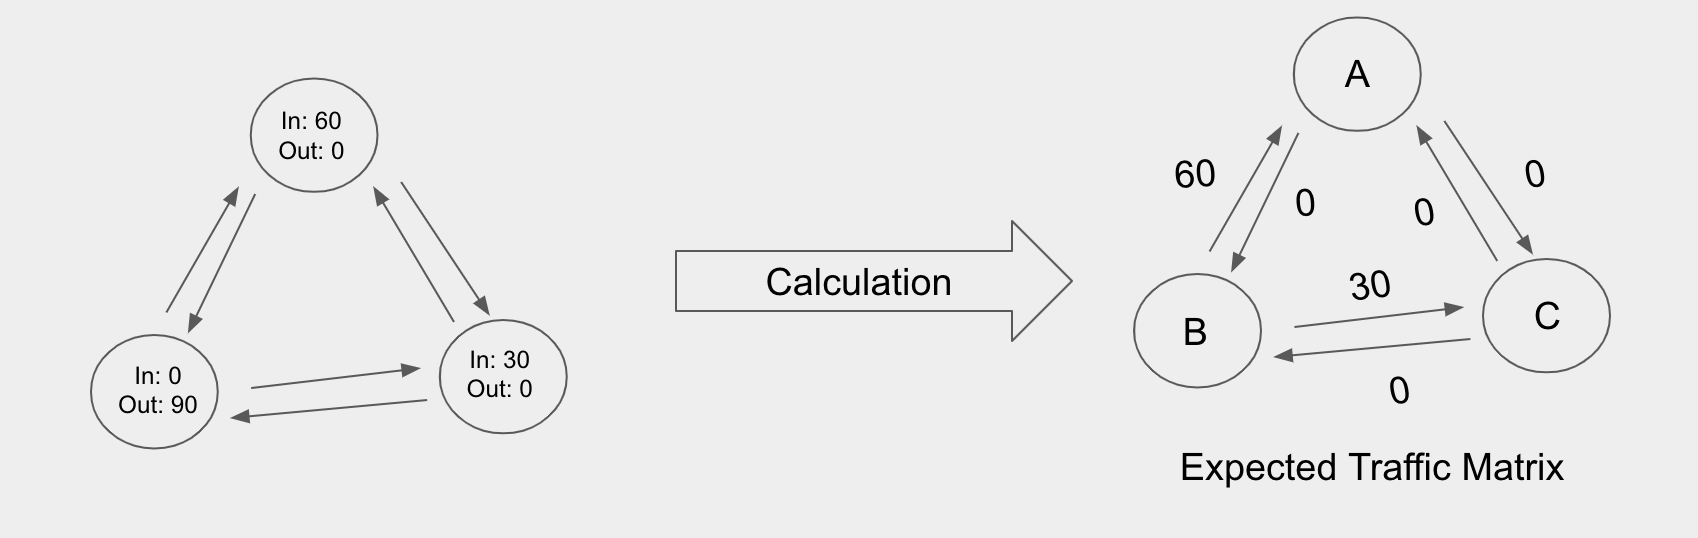
\includegraphics[width=10cm]{img/Simple_evaluation.png}
    \caption{Evaluation in Very Simple Case}
    \label{fig:eval_simple} 
\end{figure}
As shown in the figure, I use the case where the node data clearly shows the destination of all traffic.
You can see my actual test code from code listings \ref{eval_code}.
The test results correctly output the expected results, and the assertion test was passed.

For the unit test, I use Google Test to test the traffic matrix generation code that I have implemented.

\subsection{Traffic Matrix Generation Errors}
Next target is to verify that the generated traffic matrix is correct.
To evaluate the generated traffic matrix, various measures of errors are used.
The purpose of this is to compare the original traffic matrix and the generated traffic on an error scale to see how well the gravity model reproduces the characteristics of the original traffic.

The measures used in this project are Mean Squared Error (MSE), Root Mean Squared Error (RMSE), Mean Absolute Error (MAE), and Mean Absolute Percentage Error (MAPE).
As functions, I used library functions from scikit-learn.
See this page for definitions of measures of errors I used for this project.\cite{scikit-learn}

The following table transforms a randomly generated 12$\times$12 traffic matrix from a uniform distribution into node data. 
Based on the node data, the traffic matrix is generated by the function I implemented. 
This randomly generated traffic matrix from a uniform distribution is taken as the true value, and I evaluate how well my traffic matrix generator represents the original features using measures of errors.
\begin{table}[H]
    \centering
      \caption{Generation Errors}
      \label{table:loss}
      \small
      \begin{tabular}{|c||l|l|l|l|l|}  \hline
        Error & Mean & Median & Std & Min & Max \\ \hline
        MSE & 632.4389 & 630.6597 & 61.1020 & 461.3056 & 815.0278 \\
        RMSE & 24.7900 & 24.7868 & 1.2391 & 20.9479 & 28.3213 \\
        MAE & 20.2920 & 20.2639 & 1.2122 & 16.2083 & 23.8056 \\
        MAPE & 1.5686+e15 & 1.3448+e15 & 1.4074+e15 & 0.6073 & 9.3512+e15 \\ \hline
      \end{tabular}
\end{table}

The MAPE results are arbitrarily large. 
This is due to a feature of MAPE, which is that when the true value is close to zero, an extremely large value is output as the result.

In this project, there is no comparison to the gravity model. 
Therefore, it is important to note that this result does not imply that the gravity model is superior for generating quantum Internet traffic.
This will be the basis for the evaluation of traffic generation models for the Quantum Internet, which will increase in the future.
%%% Local Variables:
%%% mode: japanese-latex
%%% TeX-master: "./thesis"
%%% End:

\chapter{Conclusion}
\label{conclusion}
\section{Conclusion}
In this research, I proposed a method for generating traffic matrices based on current Internet methods, and implemented it in a Quantum Internet simulator.



%%% Local Variables:
%%% mode: japanese-latex
%%% TeX-master: "../thesis"
%%% End:


\vspace{-5mm}

\nocite{*}
\input{bib/biblio}\thispagestyle{plain}%bibtex

\chapter*{Acknowledgment}
\addcontentsline{toc}{chapter}{Acknowledgment}
\label{thanks}
First of all, I express my deepest gratitude to my advisor, Professor Rodney Van Meter.
The professor gave me a lot of advice and cared about me.
I feel very honored and blessed to have had the opportunity to study in Rod-san's seminars for 4 years.

I would like to thank the project lecturer Takahiko Satoh and the project assistant professor Michal Hajduˇsek, a faculty member in the same research group AQUA.
Thank you for mentoring me.

I would like to thank Naphan Benchasattabuse, my mentor in this thesis.
Whenever I asked a question, the answer always exceeded my expectations. 
He is a great mentor and I respect him very much.

I would also like to thank Takaaki Matsuo, Shin Nishio, Ryosuke Satoh and Yasuhiro Ohkura.
I am grateful for kind mentoring as a senior member of AQUA.
I definitely carry on the “Oi” as a AQUA tradition.

I would also like to thank my seminar colleagues, Makoto Nakai and Shigetora Miyashita.
It was a great pleasure to study quantum information and work on the same project together.

I would also like to thank Ai Toma, Shota Kusudo, Kengo Kumon, Yuta Morofuji, Yosuke Suda and Yu Yoshida.
They provided me with food, clothing and shelter for me. 
Without them, I could not have submitted my thesis.

Lastly, I would like to thank my family for bringing me up.
%%% Local Variables:
%%% mode: japanese-latex
%%% TeX-master: "../yummy_bthesis"
%%% End:

\appendix
\chapter{Appendix}

\section{Traffic Matrix Generation with Gravity Model Code for QUISP}
\begin{lstlisting}[language=c++,caption=Gravity Generator Function]
  void Application::gravityGenerator() {
    int traffic_ini = par("TrafficIni");
    int res;
    double res_all = 0;
  
    cTopology *topo = new cTopology("topo");
    topo->extractByParameter("nodeType", provider.getQNode()->par("nodeType").str().c_str());
  
    for (int i = 0; i < other_end_node_addresses.size(); i++) {
      cTopology::Node *node = topo->getNode(i);
      auto app_module = node->getModule()->getModuleByPath(".app");
      if (app_module == nullptr) throw cRuntimeError("app module not found");
      res = app_module->par("TrafficRes");
      res_all += res;
    }
    for (int i = 0; i < other_end_node_addresses.size(); i++) {
      cTopology::Node *node = topo->getNode(i);
      auto app_module = node->getModule()->getModuleByPath(".app");
      if (app_module == nullptr) throw cRuntimeError("app module not found");
      res = app_module->par("TrafficRes");
      traffic_matrix.push_back((int)round(traffic_ini * (res / res_all)));
    }
    int sum = std::accumulate(traffic_matrix.begin(), traffic_matrix.end(), 0);
    while (sum != traffic_ini) {
      std::vector<int>::iterator iter = std::max_element(traffic_matrix.begin(), traffic_matrix.end());
      size_t max_index = std::distance(traffic_matrix.begin(), iter);
      if (sum > traffic_ini) {
        traffic_matrix[max_index] -= 1;
      } else if (traffic_ini < sum) {
        traffic_matrix[max_index] += 1;
      }
      sum = std::accumulate(traffic_matrix.begin(), traffic_matrix.end(), 0);
    }
  
    delete topo;
  }
  \end{lstlisting}
  
  \begin{lstlisting}[language=c++,caption=inside of initialize function]
  if (traffic_pattern == 3) {
      gravityGenerator();
      for (int i = 0; i < other_end_node_addresses.size(); i++) {
          EV_INFO << traffic_matrix[i] << " requests will be sent from " << my_address << " to " << other_end_node_addresses[i] << "\n";
          printf("%d requests will be sent from %d to %d\n", traffic_matrix[i], my_address, other_end_node_addresses[i]);
      }
      return;
  }
  \end{lstlisting}
  

\section{Gravity Model Sample Code with Python}

\begin{lstlisting}[language=python,caption=Generate Simple Network with Python]
#Author: Nozomi Tanetani
import networkx as nx
import numpy as np
import matplotlib.pyplot as plt 

def graph_generator(n, p, seed):
  g = nx.random_graphs.fast_gnp_random_graph(n, p, seed, directed = True) #Generate a random graph
  g = g.to_undirected()

  #Initialize a number of traffic per node as 0.
  for i in g.nodes():
    g.nodes[i]['in'] = 0
    g.nodes[i]['out'] = 0

  #Store a random number into number of traffic variable.
  for i in g.nodes():
    g.nodes[i]['in'] = np.random.randint(n*100,n*500)
    tmp = g.nodes[i]['in']
    for j in g.nodes():
      if i is not j:
        if j is n-1:
          g.nodes[j]['out'] += tmp
        else:
          rand_tmp = np.random.randint(0,tmp)
          g.nodes[j]['out'] += rand_tmp
          tmp = tmp - rand_tmp
  return g

g = graph_generator(4, 1, 13)

#Display a generated graph
plt.figure(figsize=(8,8))

pos = nx.circular_layout(g)
nx.draw_networkx_nodes(g, pos, node_size=5500, node_color='gray')
nx.draw_networkx_edges(g, pos)
nx.draw_networkx_labels(g, pos, font_size=20)

#Display
labeldict = nx.get_node_attributes(g,'in')
for i in g.nodes():
  labeldict[i] = '\n\n' + str(labeldict[i])
nx.draw_networkx_labels(g,pos,labels=labeldict,font_size=12,font_color='#FFAAAA')

labeldict = nx.get_node_attributes(g,'out')
for i in g.nodes():
  labeldict[i] = '\n\n\n\n' + str(labeldict[i])
nx.draw_networkx_labels(g,pos,labels=labeldict,font_size=12,font_color='#AAFFFF')
print("red number is total traffic that enters the node.")
print("blue number is total traffic that exits the node.")
plt.show()
\end{lstlisting}

\begin{lstlisting}[language=python,caption=Gravity Generator Function with Python]
def gravity_generator(graph):
    tm = np.zeros((n,n))

    for i in range(len(tm)):
        for j in range(len(tm[i])):
        if i is not j:
            tmp = 0
            for k in range(n):
            if k is not i:
                tmp += graph.nodes[k]['out']
            tm[i][j] = int(np.round(graph.nodes()[i]['in'] * (graph.nodes[j]['out'] / tmp))) # Slide Page 15
    for i in range(len(tm)):
        if sum(tm[i]) - graph.nodes()[i]['in'] == 1:
        tm[i][np.argmax(tm[i])] -= 1
        elif graph.nodes()[i]['in'] - sum(tm[i]) == 1:
        tm[i][np.argmax(tm[i])] += 1
    return tm

#Create a traffic matrix
tm = gravity_generator(g)
print(tm)
\end{lstlisting}


\end{document}

%%% Local Variables:
%%% mode: japanese-latex
%%% TeX-master: t
%%% End: